\chapter{Introduction}
La \textbf{cinématique} est la branche de la physique qui décrit le mouvement des objets, mais elle n'étudie pas les causes de ceux-ci.

\begin{itemize}
      \item Pourquoi un mobile au repos se met-il en mouvement ?
      \item Pourquoi un corps en mouvement finit-il par s'arrêter ?
\end{itemize}

Un élément de réponse est déjà connu : si un corps se met en mouvement ou s'il s'arrête, c'est parce qu'il accélère ou parce qu'il freine.
Les situations ci-dessous présentent des cas simples d'accélération ou de décélération, précise à chaque fois la cause de celle-ci.



\begin{itemize}[$\Rightarrow$]
      \item Les wagons d'un train au repos commencent à bouger lorsque le train démarre.
            \pointilles{2}
      \item Un meuble qu'on pousse commence à bouger.
            \pointilles{2}
      \item Un objet tombe en chute libre vers la Terre.
            \pointilles{2}
      \item Un aimant se déplace lorsqu'on approche un autre aimant.
            \pointilles{2}
      \item Un vélo qui freine.
            \pointilles{2}
\end{itemize}

Dans tous les exemples, il y a un objet qui agit sur un autre. Cette interaction entre deux corps peut être caractérisée par une \motcle{force}.
\begin{encadre}
      Une force est une grandeur vectorielle qui permet de caractériser l'interaction entre deux corps.

      Force : F [Newton ; N]
\end{encadre}

La branche de la physique qui étudie les forces et leurs effets sur les corps est appelée \motcle{dynamique}. Elle permet donc d'expliquer, entre autre, la cause des mouvements.

\newpage

En 1726, Isaac newton publie la troisième version de son livre \enquote{Philosophiae naturalis principia mathematica} dans lequel il pose les bases de toute la mécanique classique aussi appelée \enquote{mécanique newtonienne}. C'est dans ce livre que figure ce que nous appelons maintenant les \enquote{trois lois de Newton}.

Ces lois sont d'une grande simplicité et constituent la base de la physique classique. Elles restent valables tant que les vitesses ne sont pas proches de celle de la lumière et que la taille des objets n'est pas proche de celle d'un électron.

La première loi, le \motcle{principe d'inertie}, explique ce qui se passe quand aucune force n'agit sur un corps.

La deuxième, la \motcle{loi fondamentale de la dynamique}, explique ce qui se passe quand une force agit sur un corps.

La troisième, le \motcle{principe des actions réciproques}, décrit les forces que deux corps en interaction exercent l'un sur l'autre.

\begin{figure}[!ht]
      \centering
      \begin{minipage}[t]{.47\linewidth}
            \centering
            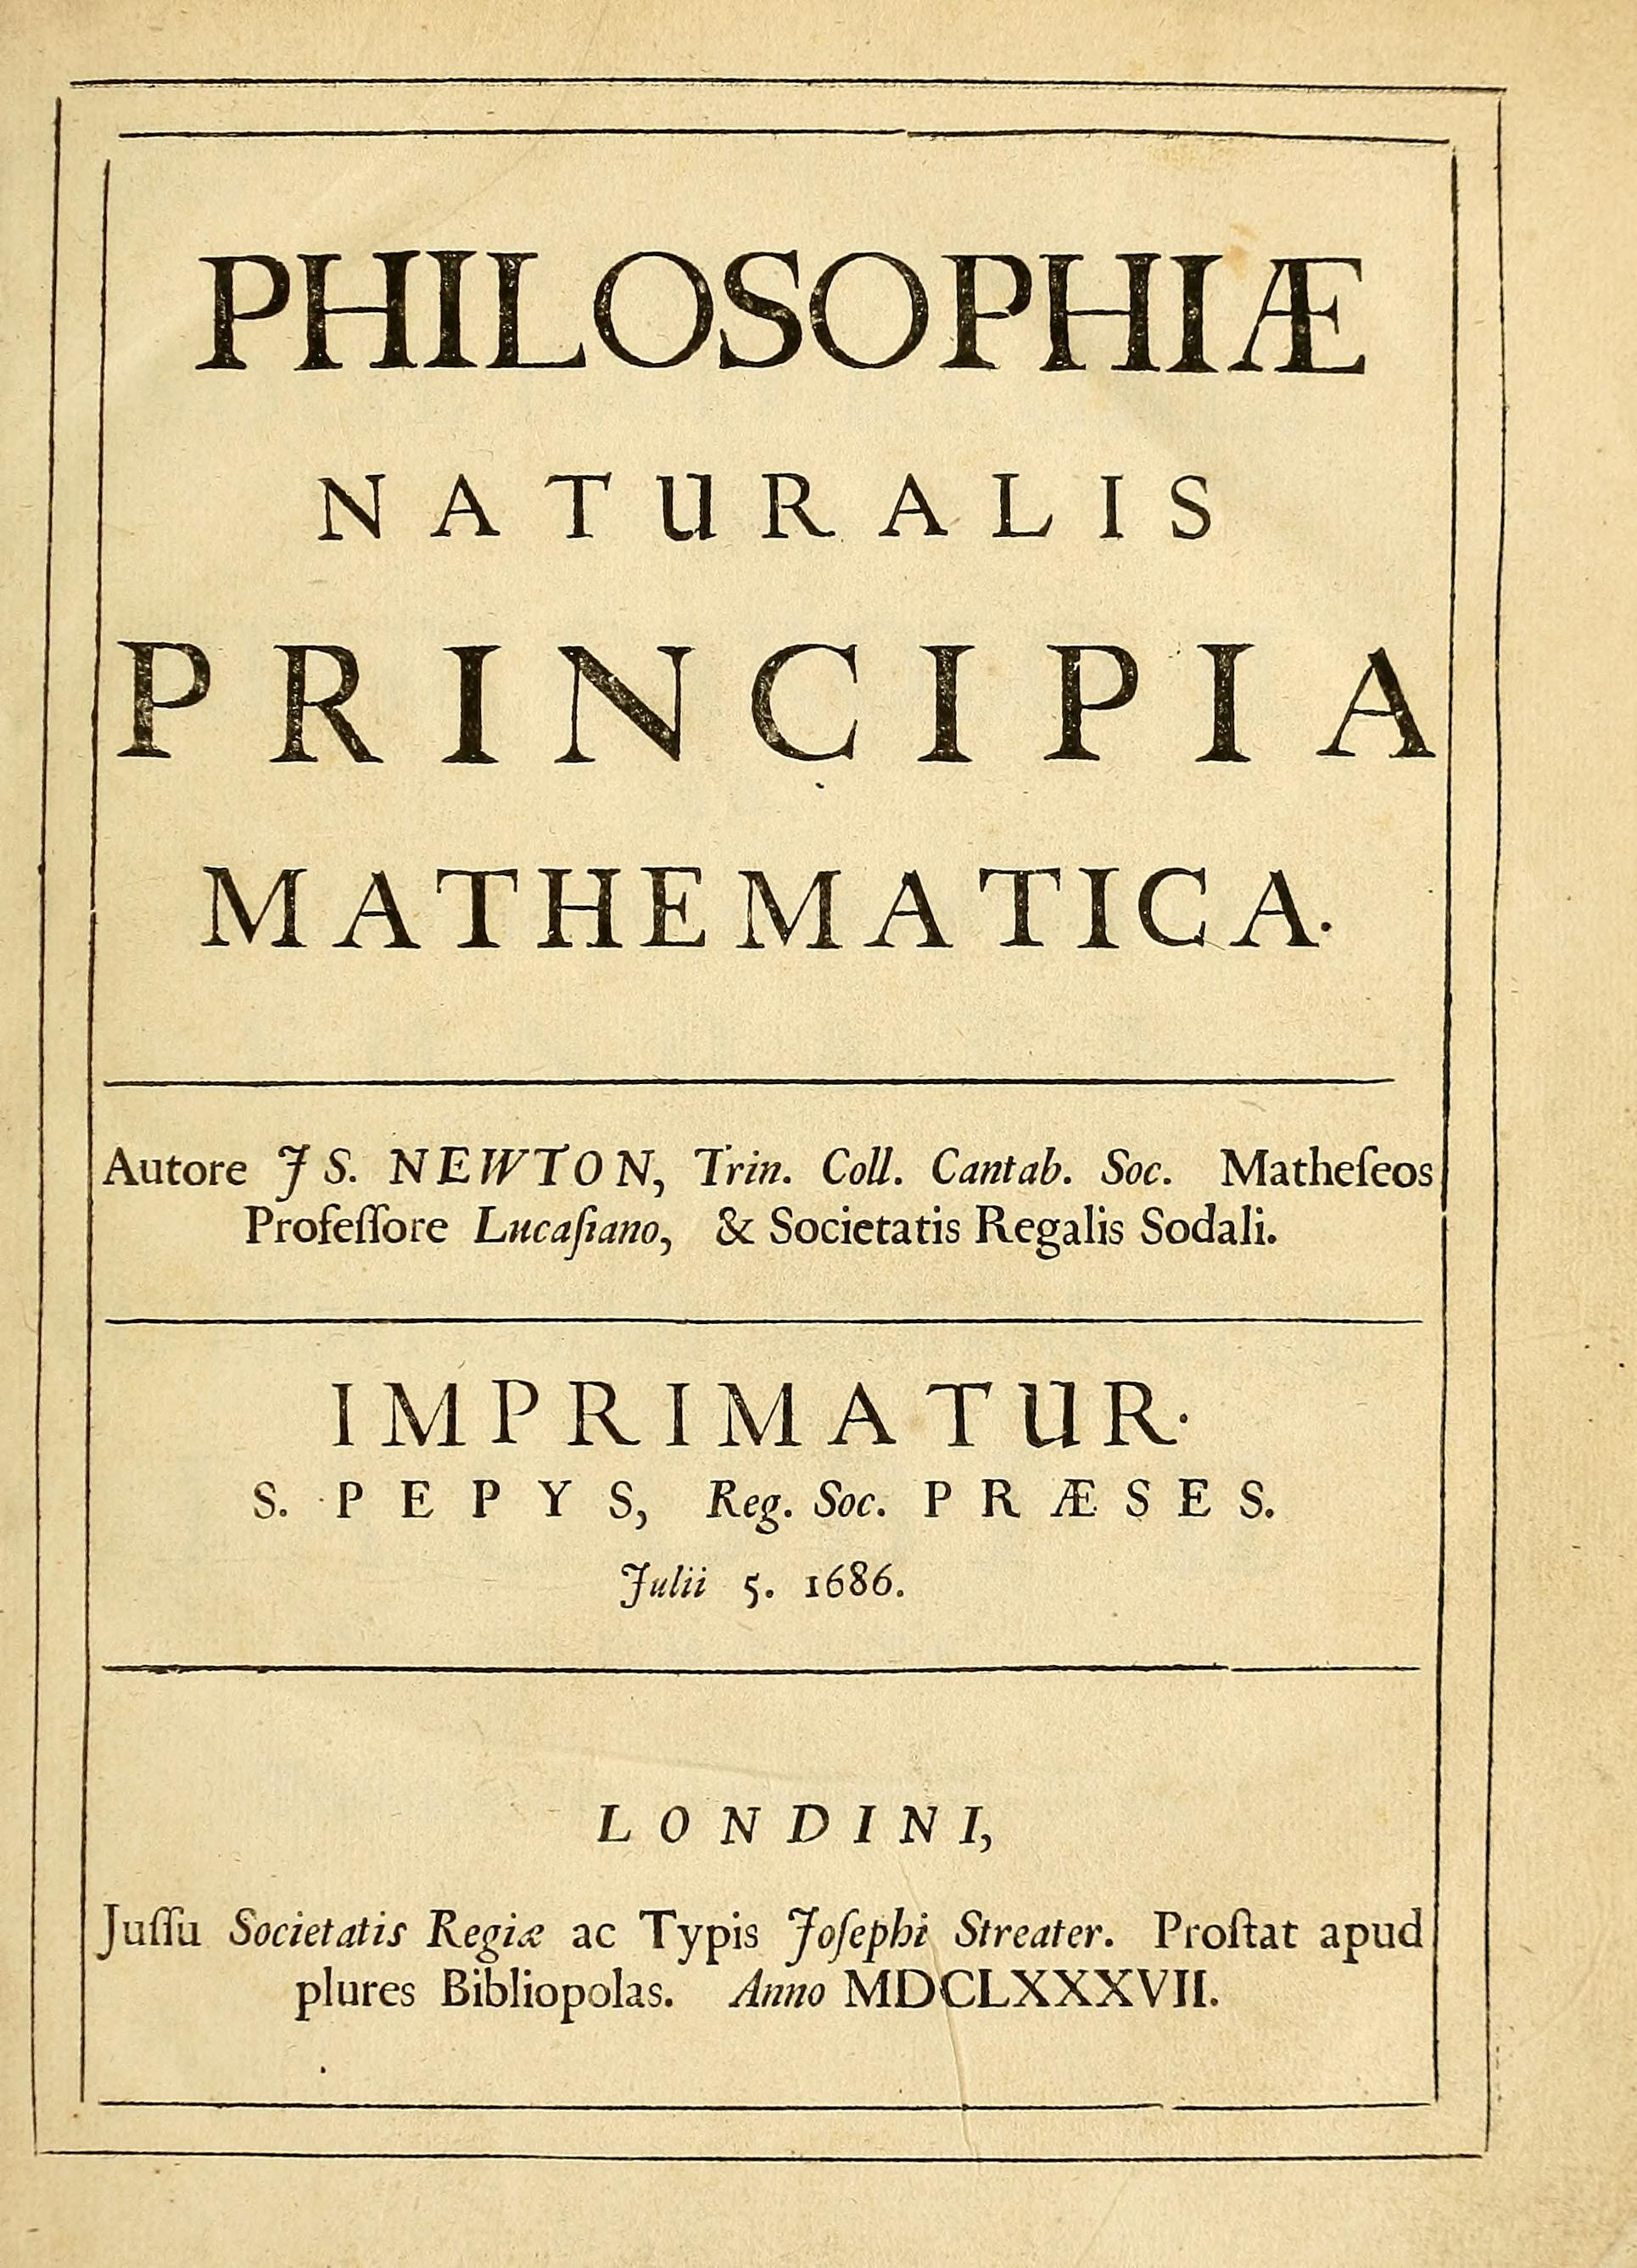
\includegraphics[width=.8 \linewidth]{Prinicipia_Newton.png}
            \caption{Page titre de Philosophiae Naturalis Principia Mathematica d'Isaac Newton, 1687.}
            \label{Prinicipia_Newton}
      \end{minipage}
      \hfill
      \begin{minipage}[t]{.47\linewidth}
            %\vspace{-\baselineskip}
            \centering
            \includegraphics[width=.8 \linewidth]{IsaacNewton-1689.jpg}
            \caption{Portrait d'Isaac Newton âgé de 46 ans par Godfrey Kneller (1689)}
            \label{IsaacNewton}
      \end{minipage}
\end{figure}

